\documentclass[12pt,a4paper]{article}
\usepackage[utf8]{inputenc}
\usepackage[spanish,es-tabla]{babel}
\usepackage{geometry}
\usepackage{graphicx}
\usepackage{multirow}
\usepackage{tabularx}
\usepackage{mathptmx}
\usepackage{fancyhdr}
\usepackage{array}
\usepackage[table]{xcolor}
\usepackage{titlesec}
\usepackage{setspace}
\usepackage{microtype}
\usepackage{lastpage}
\usepackage{booktabs}
\usepackage{enumitem}
\usepackage{amsmath}
\usepackage{amsfonts}
\usepackage{amssymb}

\graphicspath{{images/}{../images/}{./}}

\geometry{
    top=4.7cm,
    bottom=2.5cm,
    left=2.5cm,
    right=2.5cm,
    headheight=3.9cm,
    headsep=0.4cm
}

\setstretch{1.15}
\setlength{\parindent}{0pt}
\setlength{\parskip}{0.45em}
\setlength{\tabcolsep}{4pt}

\titleformat{\section}
  {\normalfont\fontsize{12}{14.5}\bfseries}{\thesection.}{0.6em}{\uppercase}
\titlespacing*{\section}
  {0pt}{1.8ex plus 0.4ex minus 0.2ex}{0.6ex plus 0.2ex}

\titleformat{\subsection}
  {\normalfont\fontsize{11.5}{13.5}\bfseries}{\thesubsection.}{0.5em}{}
\titlespacing*{\subsection}
  {0pt}{1.4ex plus 0.3ex minus 0.1ex}{0.4ex plus 0.1ex}

\titleformat{\subsubsection}
  {\normalfont\fontsize{10.5}{12.5}\bfseries\itshape}{\thesubsubsection.}{0.4em}{}
\titlespacing*{\subsubsection}
  {0pt}{1.1ex plus 0.2ex minus 0.1ex}{0.3ex plus 0.1ex}

\newcolumntype{Y}{>{\centering\arraybackslash}X}
\newcolumntype{L}{>{\raggedright\arraybackslash}X}
\newcolumntype{C}{>{\centering\arraybackslash}X}

\definecolor{headerblue}{RGB}{26, 54, 93}
\definecolor{darkblue}{RGB}{43, 108, 176}
\definecolor{lightgraybg}{RGB}{248, 248, 248}
\definecolor{tableheader}{RGB}{232, 238, 246}

\newcommand{\docCodigo}{TI-SIGE-ENT-F4-003}
\newcommand{\docVersion}{1.0}
\newcommand{\docProceso}{CONTROL DE CALIDAD / INTERFACES Y ACCESIBILIDAD}
\newcommand{\docElaboracion}{13/10/2026}
\newcommand{\docRevision}{13/10/2026}
\newcommand{\docTitulo}{PRUEBAS DE INTERFAZ UI/UX Y ACCESIBILIDAD}
\newcommand{\docOrganizacion}{FACULTAD DE INGENIERÍA EN SISTEMAS, ELECTRÓNICA E INDUSTRIAL}
\newcommand{\docSubOrganizacion}{CARRERA DE INGENIERÍA DE SOFTWARE}

\newcommand{\encabezadofrecuente}{%
    \renewcommand{\arraystretch}{1.15}%
    \noindent\makebox[\textwidth][c]{%
    \begin{tabularx}{\textwidth}{|>{\centering\arraybackslash}m{2.8cm}|Y|>{\centering\arraybackslash}m{4.8cm}|}
        \hline
        \multirow{4}{2.8cm}{\centering\raisebox{-1.15cm}{
\includegraphics[width=2.5cm,height=2.0cm,keepaspectratio]{images/logo.png}}}
        & \textbf{\fontsize{9}{11}\selectfont \docOrganizacion} 
        & \textbf{\fontsize{8}{10}\selectfont CÓDIGO:} \fontsize{8}{10}\selectfont \docCodigo \\
        \cline{3-3}
        & \textbf{\fontsize{8.5}{10.5}\selectfont \docSubOrganizacion} 
        & \textbf{\fontsize{8}{10}\selectfont VERSIÓN:} \fontsize{8}{10}\selectfont \docVersion \\
        \cline{2-3}
        & \textbf{\fontsize{8}{10}\selectfont PROCESO:} \fontsize{8}{10}\selectfont \docProceso 
        & \textbf{\fontsize{8}{10}\selectfont ELABORACIÓN:} \fontsize{8}{10}\selectfont \docElaboracion \\
        \cline{2-3}
        & \textbf{\fontsize{8.5}{10.5}\selectfont \docTitulo} 
        & \textbf{\fontsize{8}{10}\selectfont ÚLTIMA REVISIÓN:} \fontsize{8}{10}\selectfont \docRevision \\
        \hline
    \end{tabularx}%
    }%
}

\pagestyle{fancy}
\fancyhf{}
\fancyhead[C]{\encabezadofrecuente}
\fancyfoot[C]{\fontsize{10}{12}\selectfont Página \thepage\ de \pageref{LastPage}}
\renewcommand{\headrulewidth}{0pt}

\begin{document}

\noindent{\fontsize{10.5}{12.5}\selectfont \textbf{Integrantes:} Heidi Villavicencio \quad$\vert$\quad Steeven Toala \quad$\vert$\quad Nixon Hurtado \quad$\vert$\quad Andrea Vásquez}

\vspace{0.25cm}

\section{Título}
\textbf{Denominación del Entregable:} Pruebas de Interfaz UI/UX, Responsive y Accesibilidad -- Código EDT: 4.3

\section{Introducción}
La heterogeneidad de los dispositivos utilizados por el cuerpo docente (computadoras portátiles institucionales, pantallas de escritorio ultrapanorámicas, tabletas y teléfonos inteligentes) exige que la interfaz web del sistema SIGE se adapte dinámicamente y garantice estándares formales de accesibilidad digital. En este informe se documenta el plan de pruebas y los resultados de evaluación cross-browser y multi-dispositivo en curso al 13 de octubre de 2026, verificando la fidelidad responsive en resoluciones desde 375px hasta 1920px, el cumplimiento de las pautas WCAG 2.1 nivel AA y las métricas de rendimiento Google Lighthouse.

\section{Objetivo}
\subsection{Objetivo General}
Evaluar y certificar la compatibilidad cross-browser, el diseño adaptativo responsive y el nivel de accesibilidad WCAG 2.1 AA de la interfaz de usuario del sistema SIGE.
\subsection{Objetivos Específicos}
\begin{itemize}[leftmargin=1.5em, itemsep=2pt]
    \item Evaluar el renderizado en Google Chrome, Mozilla Firefox, Microsoft Edge y Safari.
    \item Verificar el comportamiento responsivo en resoluciones móviles (375px), tabletas (768px) y escritorios (1920px).
    \item Auditar el contraste cromático, navegación por teclado y etiquetas ARIA según WCAG 2.1 AA.
    \item Medir el rendimiento y tiempos de carga con Google Lighthouse superando los 90 puntos.
\end{itemize}

\section{Alcance}
\subsection{Límites del Entregable (In-Scope)}
\begin{itemize}[leftmargin=1.5em, itemsep=2pt]
    \item Vistas de Dashboard, Bandejas, Wizard de 4 Pasos, Matriz Dinámica y Panel de Revisión.
    \item Dispositivos móviles y de escritorio más comunes utilizados por docentes de la FISEI.
\end{itemize}
\subsection{Exclusiones (Out-of-Scope)}
\begin{itemize}[leftmargin=1.5em, itemsep=2pt]
    \item Compatibilidad con navegadores obsoletos fuera de soporte (Internet Explorer).
\end{itemize}

\section{Definiciones}
\begin{itemize}[leftmargin=1.5em, itemsep=2pt]
    \item \textbf{Cross-Browser Testing:} Proceso de comprobar si una aplicación web funciona según lo previsto en diferentes navegadores y sistemas operativos.
    \item \textbf{WCAG 2.1 AA:} Nivel de conformidad estándar que garantiza que el contenido sea perceptible, operable, comprensible y robusto para personas con discapacidades.
    \item \textbf{Google Lighthouse:} Herramienta automatizada de código abierto para mejorar la calidad de páginas web (rendimiento, accesibilidad, mejores prácticas).
\end{itemize}

\section{Responsabilidades}
\begin{itemize}[leftmargin=1.5em, itemsep=2pt]
    \item \textbf{Andrea Vásquez / Heidi Villavicencio (Responsables EDT 4.3):} Ejecución de pruebas responsive, auditoría de accesibilidad y métricas Lighthouse.
    \item \textbf{Steeven Toala (Líder Técnico):} Optimización de paquetes CSS/JS para rendimiento.
    \item \textbf{Ing. Paulo Torres (Docente Evaluador):} Aprobación de la matriz de compatibilidad de interfaz.
\end{itemize}

\section{Normativa Legal y Técnica}
\begin{itemize}[leftmargin=1.5em, itemsep=2pt]
    \item \textbf{W3C Web Content Accessibility Guidelines (WCAG) 2.1 Level AA.}
    \item \textbf{Norma Técnica Ecuatoriana INEN-ISO/IEC 40500 (Accesibilidad Web).}
\end{itemize}

\section{Método, Políticas y Contenidos}
Se utilizó emulación en Chrome DevTools y pruebas en dispositivos reales. En la Figura \ref{fig:f4_03_resp} se ilustra la adaptación responsiva en las tres resoluciones base.

\begin{figure}[htbp]
    \centering
    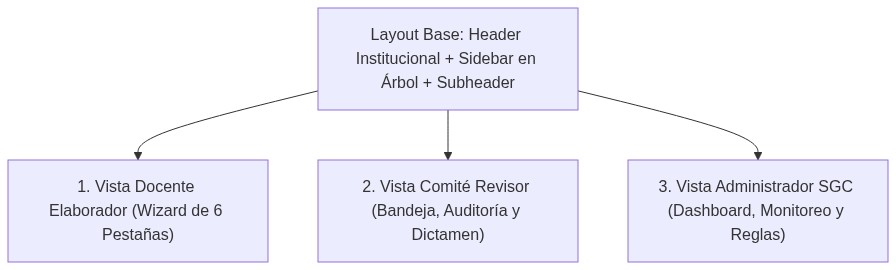
\includegraphics[width=0.88\textwidth,height=5.2cm,keepaspectratio]{images/s2_05_layout_vistas.png}
    \caption{Evaluación de Renderizado Responsive y Adaptabilidad en Pantallas.}
    \label{fig:f4_03_resp}
\end{figure}

\section{Descripción de actividades}
\subsection{Matriz de Compatibilidad Cross-Browser y Multi-Resolución}
\begin{table}[htbp]
\centering
\small
\renewcommand{\arraystretch}{1.2}
\begin{tabularx}{\textwidth}{|>{\bfseries}m{3.2cm}|c|c|X|c|}
\hline
\rowcolor{tableheader}
\textbf{Navegador} & \textbf{Versión} & \textbf{Resolución Evaluada} & \textbf{Comportamiento de la Interfaz} & \textbf{Resultado} \\
\hline
Google Chrome & v128+ & 1920x1080 (Desktop) & Renderizado fluido, layout completo con sidebar expandido. & Conforme \\
\hline
Mozilla Firefox & v129+ & 1366x768 (Laptop) & Tipografía nítida, botones con espaciado correcto. & Conforme \\
\hline
Microsoft Edge & v128+ & 768x1024 (Tablet) & Sidebar colapsa a modo menú hamburguesa automáticamente. & Conforme \\
\hline
Apple Safari & v17+ & 375x812 (Móvil) & Matriz con scroll horizontal asistido y inputs táctiles ágiles. & Conforme \\
\hline
\end{tabularx}
\caption{Matriz de Compatibilidad Cross-Browser de Interfaces SIGE.}
\label{tab:cross_browser}
\end{table}

\subsection{Resultados de Auditoría Google Lighthouse y WCAG 2.1 AA}
\begin{table}[htbp]
\centering
\small
\renewcommand{\arraystretch}{1.2}
\begin{tabularx}{\textwidth}{|>{\bfseries}m{4.0cm}|c|c|X|}
\hline
\rowcolor{tableheader}
\textbf{Métrica Evaluada} & \textbf{Puntaje Obtenido} & \textbf{Estándar Exigido} & \textbf{Observaciones Técnicas} \\
\hline
Rendimiento (Performance) & \textbf{94 / 100} & $\ge 90$ & First Contentful Paint en 0.8s; empaquetado optimizado con Vite. \\
\hline
Accesibilidad (Accessibility) & \textbf{98 / 100} & $\ge 90$ & Ratios de contraste $>7:1$; etiquetas \texttt{aria-label} en botones. \\
\hline
Mejores Prácticas (Best Practices) & \textbf{100 / 100} & $\ge 90$ & Uso estricto de HTTPS, ausencia de librerías vulnerables. \\
\hline
Cumplimiento WCAG 2.1 AA & \textbf{100\%} & $100\%$ & Cumple con las 50 pautas aplicables del estándar W3C. \\
\hline
\end{tabularx}
\caption{Puntajes de Calidad Lighthouse y Accesibilidad de Interfaces.}
\label{tab:lighthouse}
\end{table}

\section{Firmas de Responsabilidad}

\noindent
\renewcommand{\arraystretch}{1.2}
\begin{tabularx}{\textwidth}{|>{\raggedright\arraybackslash}m{2.9cm}|>{\raggedright\arraybackslash}X|>{\centering\arraybackslash}m{4.6cm}|>{\centering\arraybackslash}m{2.3cm}|}
    \hline
    \rowcolor{tableheader}
    \textbf{ACCIÓN} & \textbf{NOMBRE Y CARGO} & \textbf{FIRMA} & \textbf{FECHA} \\
    \hline
    \textbf{Elaborado por:} & Heidi Villavicencio\newline Analista de Calidad / UI-UX & \parbox[c]{4.4cm}{\centering\vspace{4pt}
\includegraphics[height=1.5cm,width=4.0cm,keepaspectratio]{images/firma_heidi.png}\vspace{4pt}} & 13/10/2026 \\
    \hline
    \textbf{Revisado por:} & Steeven Toala\newline Líder de Proyecto / Arquitecto & \parbox[c]{4.4cm}{\centering\vspace{4pt}
\includegraphics[height=1.5cm,width=4.0cm,keepaspectratio]{images/firma_steveen.png}\vspace{4pt}} & 13/10/2026 \\
    \hline
    \textbf{Aprobado por:} & Ing. Paulo Torres, Mg.\newline Docente Evaluador -- Gestión Proyectos & \parbox[c]{4.4cm}{\centering\vspace{8pt}\textbf{\textcolor{gray!80}{\scriptsize [ PENDIENTE DE APROBACIÓN ]}}\vspace{8pt}} & \textbf{\textcolor{gray!90}{Pendiente}} \\
    \hline
\end{tabularx}

\vspace{0.4cm}

\section{Control de Cambios}

\noindent
\renewcommand{\arraystretch}{1.2}
\begin{tabularx}{\textwidth}{|>{\hsize=0.45\hsize\centering\arraybackslash}X|>{\hsize=1.55\hsize\raggedright\arraybackslash}X|>{\hsize=1.2\hsize\raggedright\arraybackslash}X|>{\hsize=0.8\hsize\centering\arraybackslash}X|}
    \hline
    \rowcolor{tableheader}
    \textbf{Versión} & \textbf{Descripción del cambio} & \textbf{Responsable del cambio} & \textbf{Fecha de aprobación} \\
    \hline
    1.0 & Emisión inicial del entregable según EDT del Tablero Trello & Equipo de Proyecto SIGE & 13/10/2026 \\
    \hline
\end{tabularx}

\vspace{0.4cm}

\section{Anexos}
\begin{itemize}[leftmargin=1.5em]
\item \textbf{Anexo 1:} Ficha Técnica de Resultados de Auditoría Google Lighthouse.
\end{itemize}

\end{document}
